\section{BGP routing table}
\label{sec:bgp}

In this section we present an evaluation of the global routing table from 2003
to 2009. The first point of our interest is to analyze the contributions of
causes to the global routing table growth. That is, we determine how well ISPs
tend to use an allocated address space and how this address space is
subdivided. The second point of interest is to analyze the contents of the BGP
routing table itself. This includes an analysis of the level of the
overlapping IP prefix announcements (i.e., how many individual prefixes are
also parts of bigger prefixes present in the same routing table). We also show
the stability of the routing table contents. For this purpose, we calculate
the time periods during which each individual prefix was visible to the
selected BGP monitor. Finally, we present an analysis of the BGP routing table
dynamics grouped by the geographical region and point out countries with the
largest number of announced prefixes.

%%%%%%%%%%%%%%%%%%%%%%%%%%%%%%%%%%%%%%%%%%%%%%%%%%%%%%%%%%%%%%%%%%%%%%%%%%%%%
%%%%%%%%%%%%%%%%%%%%%%%%%%%%%%%%%%%%%%%%%%%%%%%%%%%%%%%%%%%%%%%%%%%%%%%%%%%%%
%%%%%%%%%%%%%%%%%%%%%%%%%%%%%%%%%%%%%%%%%%%%%%%%%%%%%%%%%%%%%%%%%%%%%%%%%%%%%
\subsection{Analysis of BGP table growth factors}
%%%%%%%%%%%%%%%%%%%%%%%%%%%%%%%%%%%%%%%%%%%%%%%%%%%%%%%%%%%%%%%%%%%%%%%%%%%%%
%%%%%%%%%%%%%%%%%%%%%%%%%%%%%%%%%%%%%%%%%%%%%%%%%%%%%%%%%%%%%%%%%%%%%%%%%%%%%
%%%%%%%%%%%%%%%%%%%%%%%%%%%%%%%%%%%%%%%%%%%%%%%%%%%%%%%%%%%%%%%%%%%%%%%%%%%%%

The BGP routing table growth is much faster than the growth of the number of
the allocated IP blocks (see Figure~\ref{fig:BGP vs RIR}). Currently, the
average number of entries in the global routing table is more than 3 times
more than the total number of allocated IP blocks. This increase has a dual
nature. Firstly, ISPs tend to subdivide allocated IP blocks into several
individual prefixes and announce them separately. For example, such behavior
is very typical for the transnational providers and providers which lend parts
of allocated address space to their customers, which, in their case,
independently announce lent IP address blocks. Secondly, various traffic
engineering techniques (traffic balancing, multihoming, etc) create situations
where the same address block is covered by several announced prefixes.

\subsubsection{IP block fragmentation}

Figure~\ref{fig:fragmentation} presents a correlation between allocated IP
blocks and announced IP prefixes. The \emph{matched} curve in the figure
represents IP blocks, which are announced in the exact form as they were
issued by the RIRs. An example of the matched prefix announcement is when an
ISP allocates a block of 1,024 IP addresses (equivalent to /22 block) and then
globally announces this block as a single /22 prefix. As one can see,
currently the number of matched prefixes accounts only 1/6$^{th}$ of the total
number of BGP entries, and this ratio is becoming even smaller as time
progresses.

\begin{figure}[htbp]
	\centering
		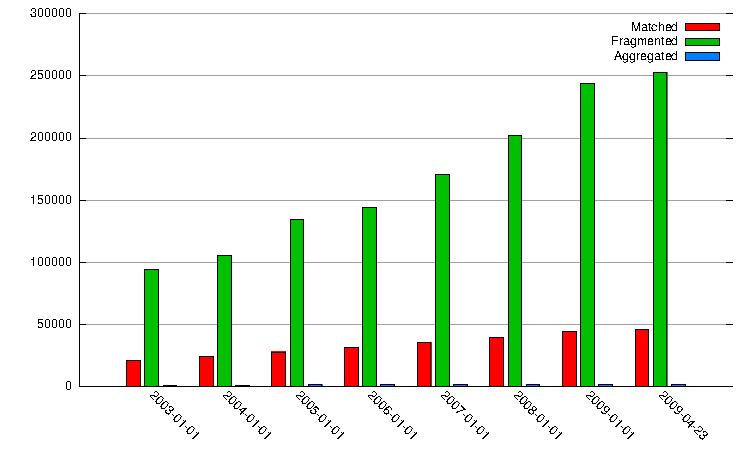
\includegraphics[width=\columnwidth]{05_matched_fragmented/frag-3}
	\caption{Dynamics of matched, fragmented, and aggregated IP prefixes in BGP announcements}
	\label{fig:fragmentation}
\end{figure}

This consideration allows us to conclude that ISPs are not willing to use
allocated address space as is. Instead, they, for some reason (e.g.,
geographical dispersion), split up allocated blocks into a number of
sub-blocks and announce each of these independently. The \emph{fragmented}
curve in Figure~\ref{fig:fragmentation} represents these split up blocks,
which accounts for more than 83\% of all entries in the global routing table.
That is, the allocated IP block fragmentation is a primary concern for
future scalability of the BGP routing table.

The last curve, \emph{aggregated}, represents IP prefix announcements, which
cover several allocated IP blocks. That is, in contrast to fragmentation,
ISPs, which have several adjacent IP block allocations, are willing to
announce them as a single IP prefix. Unfortunately, this aggregation
technique, aimed to reduce hiking the number of entries in the routing table
does not work. In 2003 the number of aggregated prefixes was 1,400 and this
number increased only marginally to nearly 2,000 prefixes in 2009, which is
nothing comparing to the total number of prefixes in the BGP routing table
($\approx$300k).

One surprising conclusion can be made from this analysis. ISPs do not tend to
globally announce the allocated IP space in the original form, no matter of
what size IP block is allocated. This conclusion can serve as a base of
different conclusion concerning future IPv6 deployment. Without a major change
in the BGP protocol, an increase of the allocation IP block size (according to
the current RIRs policy, the minimum allocation for an IPv6 block is
/32\cite{APNIC:2009:IPv6-Address} which costs the same as a /19 or /20 IPv4
address block \cite{ARIN:2009:Annual-Fee-Scedule}) will not help to
significantly reduce the size of global routing table. The only targets for
the reduction are matched IP prefixes (i.e., ISPs which currently use all
allocated IP space as a single block will likely to use a bigger IPv6 space
also as a single block). That is, the upper bound of IP space level
optimization is limited by the number of matched prefixes (less than 17\% of
all prefixes).

\subsubsection{Duplicate announcements of IP blocks}

The BGP routing table has a consistent trend of containing a large portion of
prefixes which duplicate each other (Figure~\ref{fig:covered}). In theory, IP
address coverage duplication in a routing table, where the actual route is
calculated by matching the destination address with the longest available
prefix, is an effective way to reduce the size of the routing table itself.
For example, consider an ISP owning a /8 address block and wanting to route
some /24 block using a different path than the rest of the block. It is much
effective to use a small duplication of address space and only two entries in
the routing table, instead of no duplication and 65,536 individual entries.

\begin{figure}[htbp]
	\centering
		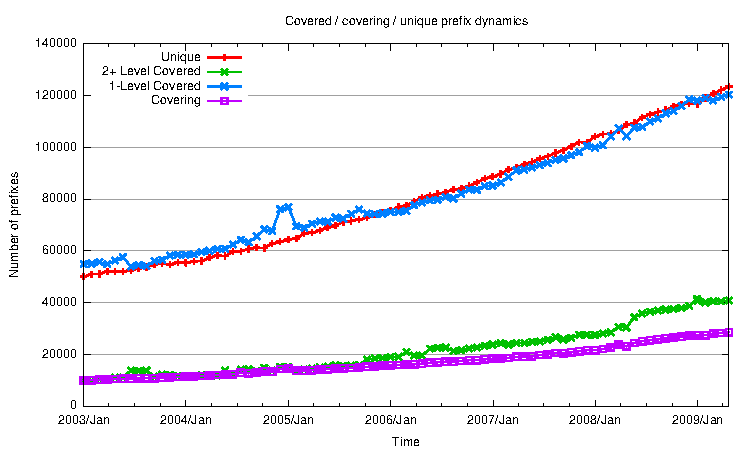
\includegraphics[width=\columnwidth]{06_covered/cover-3}
	\caption{Dynamics of covered, covering, and unique IP prefixes in BGP announcements}
	\label{fig:covered}
\end{figure}

The reality shows that the fundamental IP routing feature of longest prefix
matching is used very extensively. As we can see in Figure~\ref{fig:covered}
(\emph{1 level} curves), the number of IP prefixes in BGP table which are
covered by exactly one bigger prefix is nearly the same as the number of
unique prefixes (i.e., base prefixes). Moreover, there is a substantial amount
of prefixes which have several layers of coverage (several duplication levels,
\emph{2+ level} curve).

These high numbers indicate the presence of some additional incentives for
prefix duplication (besides the theoretical routing table optimization). One
such factor is a multi-provider connection for end-networks (so-called
multihoming of \emph{stub networks}). According to Oliveira et al.
\cite{Oliveira:2007:Observing-the-evolution}, more than 70\% of all
announcements belong to multihomed stub networks. In other words, the global
routing table was adopted to serve local or semi-local routing interests of
the majority of customers. It is very unlikely that a customer (a stub
network) connects to providers which are spaced far from each other in the
terms of routing. The conclusion is that if we want to significantly reduce
the size of the BGP routing table, we should find ways to eliminate IP prefix
fragmentation incentives. For example, separate means for multihoming and
traffic engineering tasks might be provided.

%%%%%%%%%%%%%%%%%%%%%%%%%%%%%%%%%%%%%%%%%%%%%%%%%%%%%%%%%%%%%%%%%%%%%%%%%%%%%
%%%%%%%%%%%%%%%%%%%%%%%%%%%%%%%%%%%%%%%%%%%%%%%%%%%%%%%%%%%%%%%%%%%%%%%%%%%%%
%%%%%%%%%%%%%%%%%%%%%%%%%%%%%%%%%%%%%%%%%%%%%%%%%%%%%%%%%%%%%%%%%%%%%%%%%%%%%
\subsection{Analysis of the BGP table contents}
%%%%%%%%%%%%%%%%%%%%%%%%%%%%%%%%%%%%%%%%%%%%%%%%%%%%%%%%%%%%%%%%%%%%%%%%%%%%%
%%%%%%%%%%%%%%%%%%%%%%%%%%%%%%%%%%%%%%%%%%%%%%%%%%%%%%%%%%%%%%%%%%%%%%%%%%%%%
%%%%%%%%%%%%%%%%%%%%%%%%%%%%%%%%%%%%%%%%%%%%%%%%%%%%%%%%%%%%%%%%%%%%%%%%%%%%%

Analysis of the BGP routing table contents reveals the current trends and
demands for the IP space. Later in this section we will show an analysis of
the announced prefix size distribution, IP prefix longevity in global BGP
announcements, and geographical distribution of the IP space.

\subsubsection{Lengths of announced IP prefixes}

Two of the most critical questions in the global routing system is what the
optimal length of IP prefix to allocate to customers is, and what the optimal
algorithm to select a right prefix to allocate is (e.g., how much space should
be reserved after allocated blocks in the case of repeated requests from
the same customer). There are a number of solutions to resolve the latter
question, including sequential and bisection allocation schemes and GAP
algorithm \cite{Wang:2007:Reduce-IP-Address}. The former question is still
an open research question.

Figure~\ref{fig:bgp prefix distribution} presents a distribution of the
announced prefix length. The majority of the global routing table entries are
/24-length prefixes (more than 53\% of entries). And during the last 6 years a
number of /24 prefixes practically doubled. At the same time, number of
actually allocated /24 blocks is 4 times smaller (see Figure~\ref{fig:IP
allocations}). This highlights one more time the fact that a very large number
of stub networks (i.e., relatively small customer networks) are using
announcements of small address blocks to implement multi-provider
connectivity.

\begin{figure}[htbp]
	\centering
		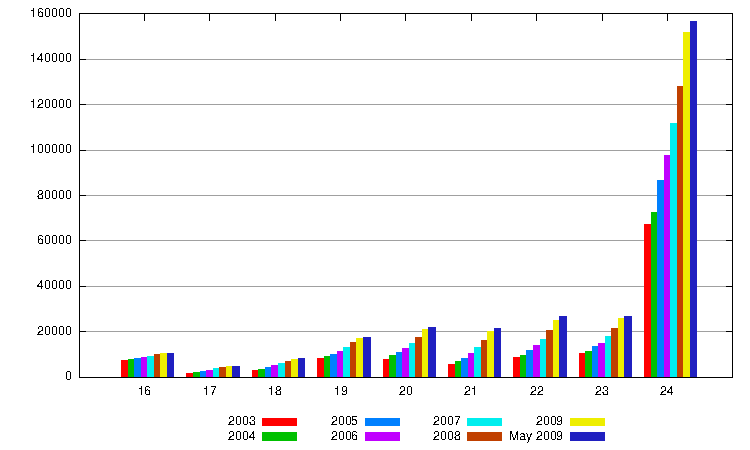
\includegraphics[width=\columnwidth]{02_prefixes/01_bgp_prefixes_zoom}
	\caption{Distribution of announced IP prefix lengths}
	\label{fig:bgp prefix distribution}
\end{figure}

Prefix length of /16 -- /23 have relatively the same level of popularity in
the global routing table, where /17 and /18 have the least popularity. The
most dynamic prefixes from this group are /20 and /21 (2.8 and 3.7 times
growth respectively), and the least dynamic -- /16 (1.4 times growth). Another
very interesting observation is for /16 prefixes. From the most influential
prefixes (in terms of the number of consuming entries in the global routing
table), the /16 prefix is the only one having the number of global
announcements practically equal to the number of allocations.

The rest of the prefixes have a marginal presence in the global routing table
(less than 8000 prefixes total). This fact shows a small number of entities
having a large (/8--/15) prefixes and a small number of a tiny customer
networks (prefixes /24--/32) with a multi-provider connectivity.

The results in this section are additional evidence of the tight
relationship between global routing table growth and IP space fragmentation
and duplication. If we can suppress the majority of non-global related
announcements (i.e., bursts of /24 prefixes due to local traffic engineering,
local and semi-local multihoming support, etc), the size of the global routing
table would be significantly reduced.

\subsubsection{Longevity distribution of BGP entries}

Another aspect of the BGP announcement analysis is determining the stability
of the global routing table. The distribution of prefix longevity is shown in
Figure~\ref{fig:bgp ages}. The main observation from the graph is that more
than 15\% of the global routing table never changes. On the other hand, about
15\% (if we compare to the global routing table size in 2009) of the prefixes
were active only for short period of time. A part of these short-lived
prefixes, probably, belongs to spammers who hijack somebody else's (or
nobody's) prefix and announce it for the time to send virtually untraceable
spam messages \cite{Ramachandran:2006:Understanding-the-network-level}. Part
of the short-lived prefixes could be explained by the configuration errors.
The rest are, probably, explained by the normal BGP operation where some
prefix become visible only in the case of a primary network channel
malfunctions.

\begin{figure}[htbp]
	\centering
		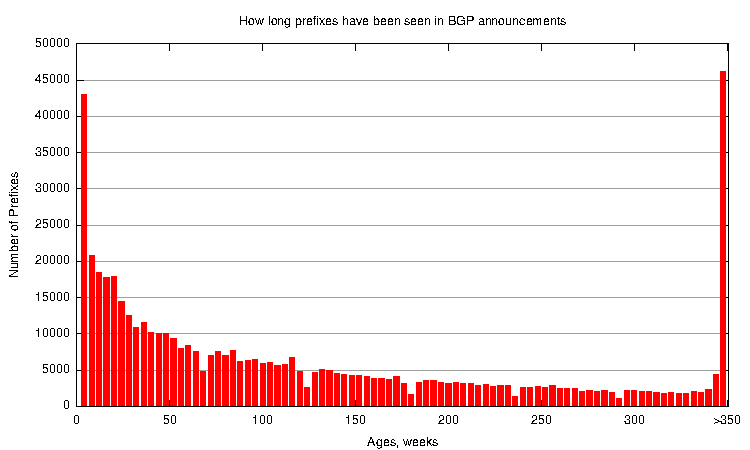
\includegraphics[width=\columnwidth]{08_ages/ages-4}
	\caption{Longevity of prefixes in BGP announcements}
	\label{fig:bgp ages}
\end{figure}

As one can see from Figure~\ref{fig:bgp ages}, the prefix longevity
distribution is to some extent following the exponential distribution
function. That is, besides a fixed number of highly stable routes (15\%), it
is unlikely that some route is visible for very long time. In other words,
announced prefixes are likely to have a small longevity. This observation
shows the substantial level of the global routing table dynamics.

\subsubsection{BGP announcements by geographical region}

As a final analysis of the global routing table content, we present a
country-based analysis for the number of globally announced IP prefixes. The
analysis of a fixed-time snapshots points out the major contributers to the
global routing table and gives an understanding of the Internet's penetration
throughout the world.

Table~\ref{tab:top25 bgp prefixes 2003} presents a top 25 contributors to the
global routing table in 2003 with the indications of what actual IP address
space is covered by the sets of announced prefixes. Table~\ref{tab:top25 bgp
ip space 2003} gives an alternative representation for the BGP data snapshot
from 2003, where countries are ordered by the number of IP addresses covered
by BGP announcements. Due to the limited nature of our IP prefix country
association technique (we matched announced address space with corresponding
allocated address space), there is a considerable portion of the prefixes for
which we could not establish such an association. In fact, in 2003 globally
announced prefixes with undetermined ownership were the second largest
contributors to the routing table after the United States. Third and forth
place for contribution to the routing table in 2003 were taken by Australia
and Canada. It should be mentioned that geographical distribution of announced
IP prefixes and announced IP space has a stable quasi-exponential distribution
(Figure~\ref{fig:prefix distr} and Figure~\ref{fig:size distr})

\begin{figure}[htbp]
	\centering
		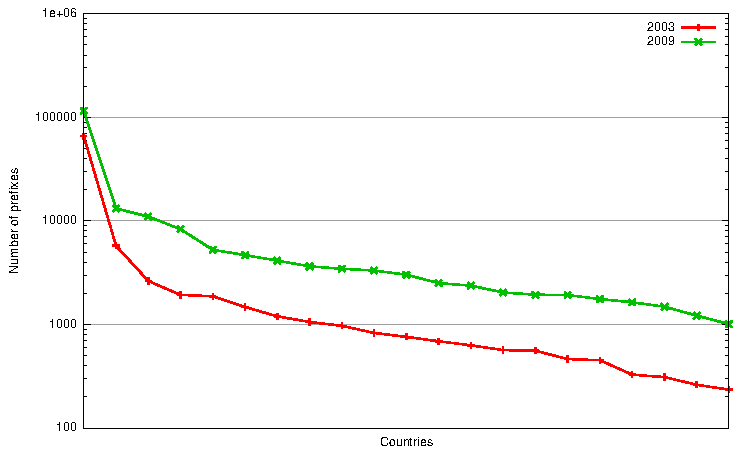
\includegraphics[width=\columnwidth]{01_bgp_ip_size/prefix-distr}
	\caption{Geographical distribution of globally announced IP prefixes (log scale)}
	\label{fig:prefix distr}
\end{figure}

\begin{figure}[htbp]
	\centering
		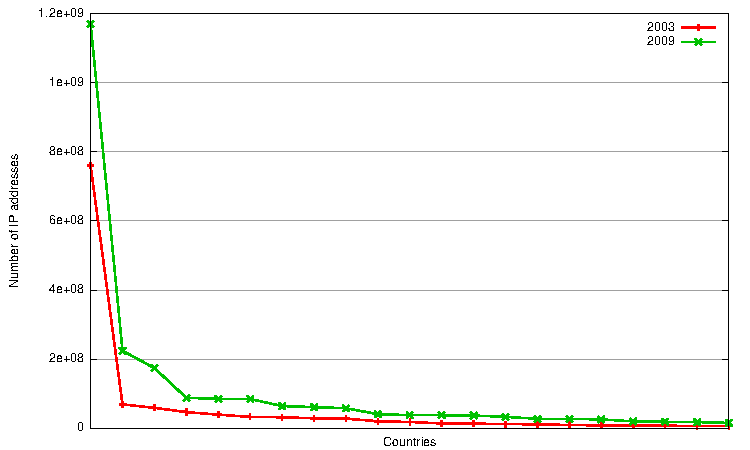
\includegraphics[width=\columnwidth]{01_bgp_ip_size/size-distr}
	\caption{Geographical distribution of globally announced IP space (log scale)}
	\label{fig:size distr}
\end{figure}

Table~\ref{tab:top25 bgp prefixes 2009} and Table~\ref{tab:top25 bgp ip space
2009} present an up-to-date estimate of the top 25 contributors to the global
routing table and the top 25 countries with the most announced address space.
As we can see, a number of prefixes with undetermined ownership (and the
corresponding IP space) decreased twice. At the same time all countries show a
substantial growth in BGP table usage. Although, the United States saved its
leading position, the rest of the table had significant changes. South Korea,
China, Australia, and India became the second major contributors to the size
of the global routing table. At the same time, China, Japan, the European
Union, Germany, and South Korea have the most announced address space. This
observation highlights the fact that some countries tend to announce a large
number of relatively small prefixes (e.g., in South Korea one prefix covers on
average 5,900 addresses), and some announce a small number of large prefixes
(e.g., in Japan one prefix covers on average 37,200 addresses). If this
difference in usage efficiency occurs because of additional government
regulations, than for future IPv6 deployment, we should consider an
establishment of similar global regulations.

 % are extremely efficient from BGP point of view

As an alternative way to represent each country's contribution to the global
routing table, we present color-coded diagrams in Figures~\ref{fig:bgp
prefixes 2003}--\ref{fig:bgp ip space asia 2009}. The figure pairs
(Figure~\ref{fig:bgp prefixes 2003} and Figure~\ref{fig:bgp prefixes 2009},
Figure~\ref{fig:bgp ip space 2003} and Figure~\ref{fig:bgp ip space 2009})
allows trace the regional Internet growth dynamics. Figure~\ref{fig:bgp
prefixes asia 2009} and Figure~\ref{fig:bgp ip space asia 2009} emphasize one
more time differences of the varying effectiveness of IP space utilization
(e.g., Japan has many more addresses per announced prefix compared to India or
South Korea).


\begin{table*}[p]
%%%%%%%%%%%%%%%%%%%%%%%%%%%%%%%%%%%%%%%%%%%%%%%%%%%%%%%%%%%%%%%%%%%%%%%%%%%%%%%%
%% TOP announced prefixes
%%%%%%%%%%%%%%%%%%%%%%%%%%%%%%%%%%%%%%%%%%%%%%%%%%%%%%%%%%%%%%%%%%%%%%%%%%%%%%%%
\begin{minipage}[t]{0.48\textwidth}
% \begin{table}[p]
	\begin{center}
	\caption{Top 25 countries with the most number of announced prefixes in BGP table on \textbf{January 1, 2003}}
	\label{tab:top25 bgp prefixes 2003}
	\begin{tabular}{|l||l|r|r|} %\hline
		\hline
		&      \bf Country		&    Prefixes   &       IP space 		\tabularnewline \hline 
1       &       US      		&       65849   &       759,792,816     \tabularnewline %\hline
2       &       \emph{Unknown}	&       6258    &       68,926,314      \tabularnewline %\hline
3       &       Australia       &       5762    &       17,822,159      \tabularnewline %\hline
4       &       Canada  		&       5612    &       38,912,924      \tabularnewline %\hline
5       &       Japan   		&       2633    &       58,905,280      \tabularnewline %\hline
6       &       South Korea     &       2441    &       27,334,687      \tabularnewline %\hline
7       &       Germany			&       1934    &       46,556,556      \tabularnewline %\hline
8       &       India  			&       1931    &       2,943,040       \tabularnewline %\hline
9       &       UK     			&       1873    &       32,626,649      \tabularnewline %\hline
10      &       China  			&       1615    &       28,522,130      \tabularnewline %\hline
11      &       Argentina       &       1477    &       2,017,448       \tabularnewline %\hline
12      &       Hong Kong       &       1261    &       5,621,473       \tabularnewline %\hline
13      &       Sweden  		&       1198    &       11,280,533      \tabularnewline %\hline
14      &       France  		&       1148    &       31,320,040      \tabularnewline %\hline
15      &       Mexico  		&       1059    &       5,275,520       \tabularnewline %\hline
16      &       Romania 		&       994     &       667,136 		\tabularnewline %\hline
17      &       Russia  		&       972     &       5,911,712       \tabularnewline %\hline
18      &       Chile   		&       834     &       2,098,161       \tabularnewline %\hline
19      &       Indonesia       &       830     &       1,170,560       \tabularnewline %\hline
20      &       Italy   		&       791     &       13,324,288      \tabularnewline %\hline
21      &       Brazil  		&       760     &       11,580,416      \tabularnewline %\hline
22      &       Taiwan  		&       708     &       13,448,168      \tabularnewline %\hline
23      &       Netherlands     &       689     &       19,939,341      \tabularnewline %\hline
24      &       European Union  &       687     &       2,707,383       \tabularnewline %\hline
25      &       Finland 		&       630     &       7,307,018       \tabularnewline %\hline
% 26      &       South Africa    &       618     &       5,762,180       \tabularnewline %\hline
% 27      &       New Zealand     &       566     &       3,828,620       \tabularnewline %\hline
% 28      &       Switzerland     &       560     &       7,937,424       \tabularnewline %\hline
% 29      &       Thailand        &       559     &       1,877,060       \tabularnewline %\hline
% 30      &       Spain   		&       511     &       8,921,568       \tabularnewline %\hline
	\hline
	\end{tabular}
	\end{center}
% \end{table}
\end{minipage}
%
\quad
%
\begin{minipage}[t]{0.48\textwidth}
% \begin{table}[p]
	\begin{center}
	\caption{Top 25 countries with the most number of announced prefixes in BGP table on \textbf{April 23, 2009}}
	\label{tab:top25 bgp prefixes 2009}
	\begin{tabular}{|l||l|r|r|r|}
		\hline
		&      \bf Country		& \bf Prefixes  &       \bf IP space 	& \bf Change$^{*}$ 	\tabularnewline \hline 
1       &       US      		&       115780  &       1,170,481,177   & 1.54			\tabularnewline %\hline
2       &       South Korea     &       14308   &       84,553,300      & 3.09			\tabularnewline %\hline
3       &       China  			&       13188   &       223,990,021     & 7.85			\tabularnewline %\hline
4       &       Australia       &       11329   &       37,818,072      & 2.12			\tabularnewline %\hline
5       &       India   		&       11022   &       17,575,040      & 5.97			\tabularnewline %\hline
6       &       Russia  		&       8650    &       26,664,224      & 4.51			\tabularnewline %\hline
7       &       Canada  		&       8328    &       57,471,348      & 1.48			\tabularnewline %\hline
8       &       Romania 		&       5729    &       7,348,881       & 11.02			\tabularnewline %\hline
9       &       UK      		&       5269    &       63,871,082      & 1.96			\tabularnewline %\hline
10      &       European Union  &       4937    &       87,825,582      & 32.44			\tabularnewline %\hline
11      &       Japan   		&       4674    &       173,789,965     & 2.95			\tabularnewline %\hline
12      &       Brazil  		&       4643    &       40,429,504      & 3.49			\tabularnewline %\hline
13      &       Argentina       &       4142    &       9,721,411       & 4.82			\tabularnewline %\hline
14      &       Germany 		&       4035    &       84,904,642      & 1.82			\tabularnewline %\hline
15      &       Mexico  		&       3648    &       19,583,832      & 3.71			\tabularnewline %\hline
16      &       Indonesia       &       3562    &       5,248,256       & 4.48			\tabularnewline %\hline
17      &       Hong Kong       &       3459    &       14,764,300      & 2.63			\tabularnewline %\hline
18      &       \emph{Unknown}	&       3393    &       37,265,411      & 				\tabularnewline %\hline
19      &       Bulgaria        &       3325    &       4,439,040       & 7.72			\tabularnewline %\hline
20      &       Colombia        &       3029    &       4,901,340       & 11.86			\tabularnewline %\hline
21      &       Ukraine 		&       3028    &       5,547,136       & 7.67			\tabularnewline %\hline
22      &       Egypt  			&       2992    &       3,854,848       & 4.60			\tabularnewline %\hline
23      &       France 			&       2511    &       61,070,996      & 1.95			\tabularnewline %\hline
24      &       Taiwan 			&       2511    &       36,623,744      & 2.72			\tabularnewline %\hline
25      &       Chile  			&       2375    &       6,101,376       & 2.91			\tabularnewline %\hline
% 26      &       Poland 			&       2341    &       15,122,881      & 4.06			\tabularnewline %\hline
% 27      &       Thailand        &       2039    &       7,210,800       & 3.84			\tabularnewline %\hline
% 28      &       Spain   		&       1989    &       25,315,136      & 2.84			\tabularnewline %\hline
% 29      &       Sweden  		&       1942    &       18,532,345      & 1.64			\tabularnewline %\hline
% 30      &       Turkey  		&       1940    &       14,309,632      & 6.41			\tabularnewline %\hline
	\hline
	\end{tabular}
	\end{center}
	
	\small	$^{*}$ -- Relative change in number of prefixes in BGP announcements from January 1, 2003 and April 23, 2009
% \end{table}
\end{minipage}

\vspace{1cm}

%%%%%%%%%%%%%%%%%%%%%%%%%%%%%%%%%%%%%%%%%%%%%%%%%%%%%%%%%%%%%%%%%%%%%%%%%%%%%%%%
%% TOP announced IP space
%%%%%%%%%%%%%%%%%%%%%%%%%%%%%%%%%%%%%%%%%%%%%%%%%%%%%%%%%%%%%%%%%%%%%%%%%%%%%%%%
\begin{minipage}[t]{0.48\textwidth}
% \begin{table}[p]
	\begin{center}
	\caption{Top 25 countries with the most number of announced IP space in BGP table on \textbf{January 1, 2003}}
	\label{tab:top25 bgp ip space 2003}
	\begin{tabular}{|l||l|r|r|}
		\hline
		&      \bf Country		&    Prefixes   &       IP space 		\tabularnewline \hline 
1       &       US      		&       65849   &       759,792,816     \tabularnewline %\hline
2       &       \emph{Unknown} 	&       6258    &       68,926,314      \tabularnewline %\hline
3       &       Japan   		&       2633    &       58,905,280      \tabularnewline %\hline
4       &       Germany 		&       1934    &       46,556,556      \tabularnewline %\hline
5       &       Canada  		&       5612    &       38,912,924      \tabularnewline %\hline
6       &       UK      		&       1873    &       32,626,649      \tabularnewline %\hline
7       &       France  		&       1148    &       31,320,040      \tabularnewline %\hline
8       &       China   		&       1615    &       28,522,130      \tabularnewline %\hline
9       &       South Korea     &       2441    &       27,334,687      \tabularnewline %\hline
10      &       Netherlands     &       689     &       19,939,341      \tabularnewline %\hline
11      &       Australia       &       5762    &       17,822,159      \tabularnewline %\hline
12      &       Taiwan  		&       708     &       13,448,168      \tabularnewline %\hline
13      &       Italy   		&       791     &       13,324,288      \tabularnewline %\hline
14      &       Brazil  		&       760     &       11,580,416      \tabularnewline %\hline
15      &       Sweden  		&       1198    &       11,280,533      \tabularnewline %\hline
16      &       Spain   		&       511     &       8,921,568       \tabularnewline %\hline
17      &       Switzerland     &       560     &       7,937,424       \tabularnewline %\hline
18      &       Norway  		&       262     &       7,591,936       \tabularnewline %\hline
19      &       Finland 		&       630     &       7,307,018       \tabularnewline %\hline
20      &       Russia  		&       972     &       5,911,712       \tabularnewline %\hline
21      &       South Africa    &       618     &       5,762,180       \tabularnewline %\hline
22      &       Hong Kong       &       1261    &       5,621,473       \tabularnewline %\hline
23      &       Austria 		&       317     &       5,405,664       \tabularnewline %\hline
24      &       Mexico  		&       1059    &       5,275,520       \tabularnewline %\hline
25      &       Denmark 		&       196     &       4,169,984       \tabularnewline %\hline
% 26      &       New Zealand     &       566     &       3,828,620       \tabularnewline %\hline
% 27      &       Belgium 		&       175     &       3,796,224       \tabularnewline %\hline
% 28      &       Poland  		&       273     &       3,721,216       \tabularnewline %\hline
% 29      &       Malaysia        &       235     &       3,182,400       \tabularnewline %\hline
% 30      &       India   		&       1931    &       2,943,040       \tabularnewline %\hline
	\hline
	\end{tabular}
	\end{center}
	\ \newline\ \newline
% \end{table}
\end{minipage}
%
\quad
%
\begin{minipage}[t]{0.48\textwidth}
% \begin{table}[p]
	\begin{center}
	\caption{Top 25 countries with the most number of announced IP space in BGP table on \textbf{April 23, 2009}}
	\label{tab:top25 bgp ip space 2009}
	\begin{tabular}{|l||l|r|r|r|}
		\hline
		&      \bf Country		& \bf Prefixes  &       \bf IP space 	& \bf Change$^{*}$ 	\tabularnewline \hline 
1       &       US      		&       115780  &       1,170,481,177   & 1.76			\tabularnewline %\hline
2       &       China   		&       13188   &       223,990,021     & 8.17			\tabularnewline %\hline
3       &       Japan   		&       4674    &       173,789,965     & 1.78			\tabularnewline %\hline
4       &       European Union  &       4937    &       87,825,582      & 7.19			\tabularnewline %\hline
5       &       Germany 		&       4035    &       84,904,642      & 2.09			\tabularnewline %\hline
6       &       South Korea     &       14308   &       84,553,300      & 5.86			\tabularnewline %\hline
7       &       UK      		&       5269    &       63,871,082      & 2.81			\tabularnewline %\hline
8       &       France  		&       2511    &       61,070,996      & 2.19			\tabularnewline %\hline
9       &       Canada  		&       8328    &       57,471,348      & 1.48			\tabularnewline %\hline
10      &       Brazil  		&       4643    &       40,429,504      & 6.11			\tabularnewline %\hline
11      &       Australia       &       11329   &       37,818,072      & 1.97			\tabularnewline %\hline
12      &       \emph{Unknown}	&       3393    &       37,265,411      & 				\tabularnewline %\hline
13      &       Taiwan  		&       2511    &       36,623,744      & 3.55			\tabularnewline %\hline
14      &       Italy   		&       1686    &       32,551,268      & 2.13			\tabularnewline %\hline
15      &       Netherlands     &       1883    &       27,122,689      & 2.73			\tabularnewline %\hline
16      &       Russia  		&       8650    &       26,664,224      & 8.90			\tabularnewline %\hline
17      &       Spain   		&       1989    &       25,315,136      & 3.89			\tabularnewline %\hline
18      &       Mexico  		&       3648    &       19,583,832      & 3.44			\tabularnewline %\hline
19      &       Sweden  		&       1942    &       18,532,345      & 1.62			\tabularnewline %\hline
20      &       India   		&       11022   &       17,575,040      & 5.71			\tabularnewline %\hline
21      &       Poland  		&       2341    &       15,122,881      & 8.58			\tabularnewline %\hline
22      &       Hong Kong       &       3459    &       14,764,300      & 2.74			\tabularnewline %\hline
23      &       Turkey  		&       1940    &       14,309,632      & 8.40			\tabularnewline %\hline
24      &       South Africa    &       1218    &       12,969,116      & 1.97			\tabularnewline %\hline
25      &       Argentina       &       4142    &       9,721,411       & 2.80			\tabularnewline %\hline
% 26      &       Vietnam        	&       1010    &       9,514,496       & 50.50			\tabularnewline %\hline
% 27      &       Switzerland     &       1230    &       9,244,448       & 2.20			\tabularnewline %\hline
% 28      &       Denmark 		&       569     &       9,239,192       & 2.90			\tabularnewline %\hline
% 29      &       Malaysia        &       572     &       8,791,684       & 2.43			\tabularnewline %\hline
% 30      &       Finland 		&       469     &       8,691,972       & 0.74			\tabularnewline %\hline
	\hline
	\end{tabular}
	\end{center}
	\small	$^{*}$ -- Relative change in globally announced IP space from January 1, 2003 and April 23, 2009
% \end{table}
\end{minipage}

\end{table*}

% \clearpage

\begin{figure*}[p]
\centering

%%%%%%%%%%%%%%%%%%%%%%%%%%%%%%%%%%%%%%%%%%%%%%%%%%%%%%%%%%%%%%%%%%
%% BGP counts
%%%%%%%%%%%%%%%%%%%%%%%%%%%%%%%%%%%%%%%%%%%%%%%%%%%%%%%%%%%%%%%%%%
\begin{minipage}[b]{0.48\textwidth}
% \begin{figure}[p]
	\centering
		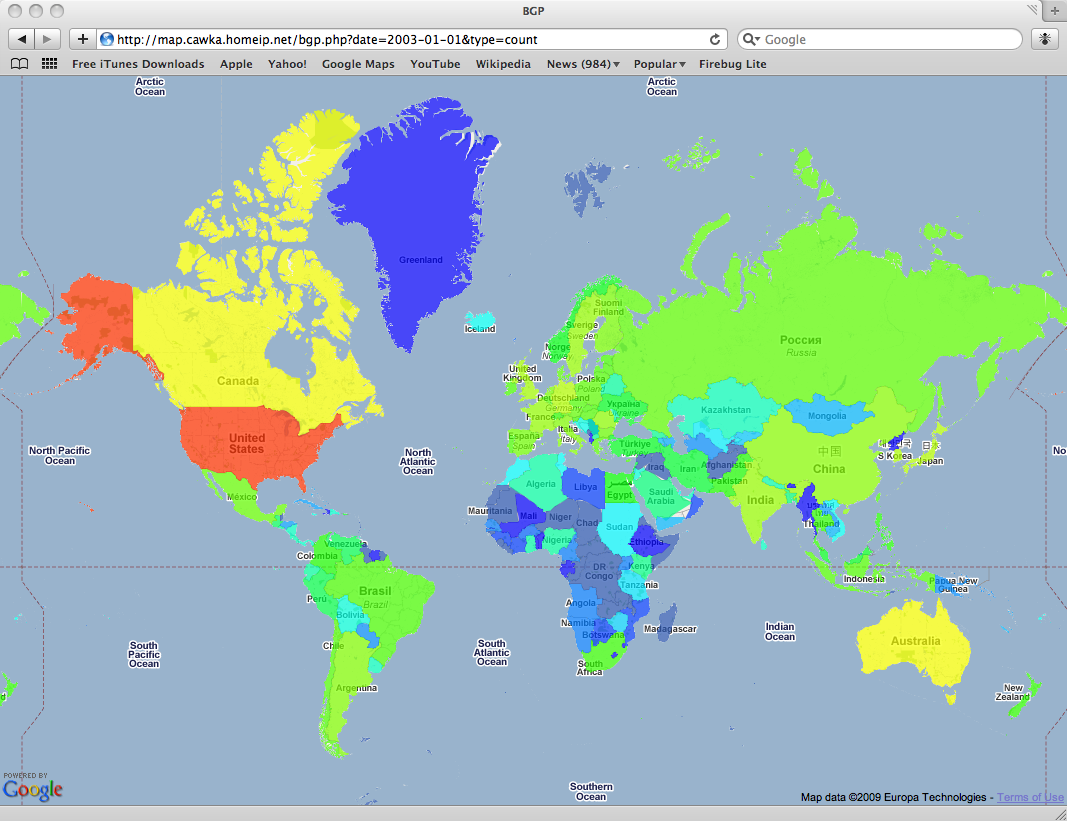
\includegraphics[trim=0 17px 0px 76px,clip=true,width=\columnwidth]{00_maps/bgp_count_2003}%
		\hspace{-0.98\columnwidth}%
		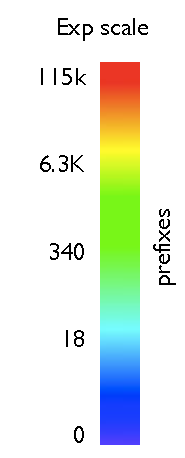
\includegraphics[width=1cm]{scale_bgp_count}\hspace{-1cm}%
		\hspace{0.98\columnwidth}
	\caption{Geographical distribution of number of announced prefixes on \textbf{January 1, 2003}}
	\label{fig:bgp prefixes 2003}
% \end{figure}
\end{minipage}%
%
\quad
%
\begin{minipage}[b]{0.48\textwidth}
% \begin{figure}[p]
	\centering
		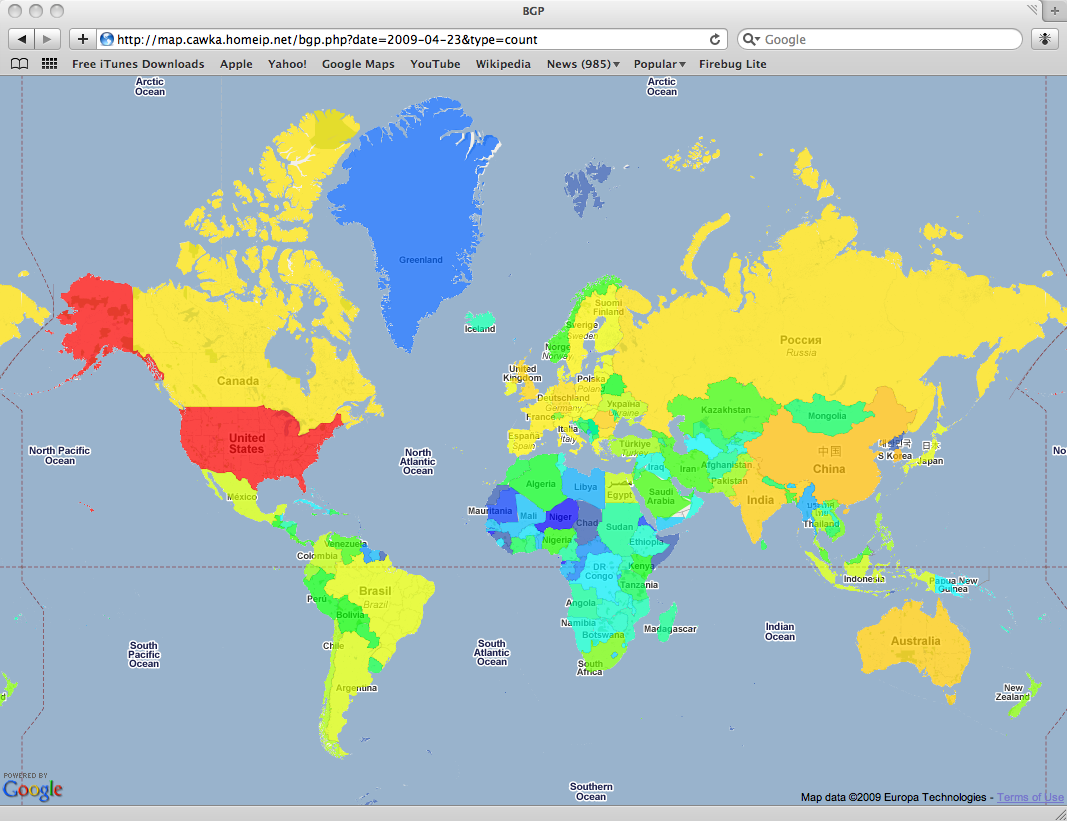
\includegraphics[trim=0 17px 0px 76px,clip=true,width=\columnwidth]{00_maps/bgp_count_2009_2}%
		\hspace{-0.98\columnwidth}%
		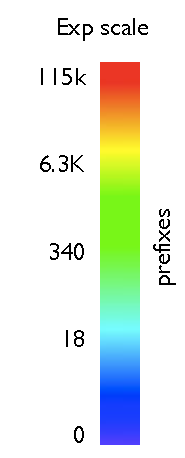
\includegraphics[width=1cm]{scale_bgp_count}\hspace{-1cm}%
		\hspace{0.98\columnwidth}
	\caption{Geographical distribution of number of announced prefixes on \textbf{April 23, 2009}}
	\label{fig:bgp prefixes 2009}
% \end{figure}
\end{minipage}

\vspace{0.5cm}

%%%%%%%%%%%%%%%%%%%%%%%%%%%%%%%%%%%%%%%%%%%%%%%%%%%%%%%%%%%%%%%%%%
%% BGP sizes
%%%%%%%%%%%%%%%%%%%%%%%%%%%%%%%%%%%%%%%%%%%%%%%%%%%%%%%%%%%%%%%%%%
\begin{minipage}[b]{0.48\textwidth}
% \begin{figure}[p]
	\centering
		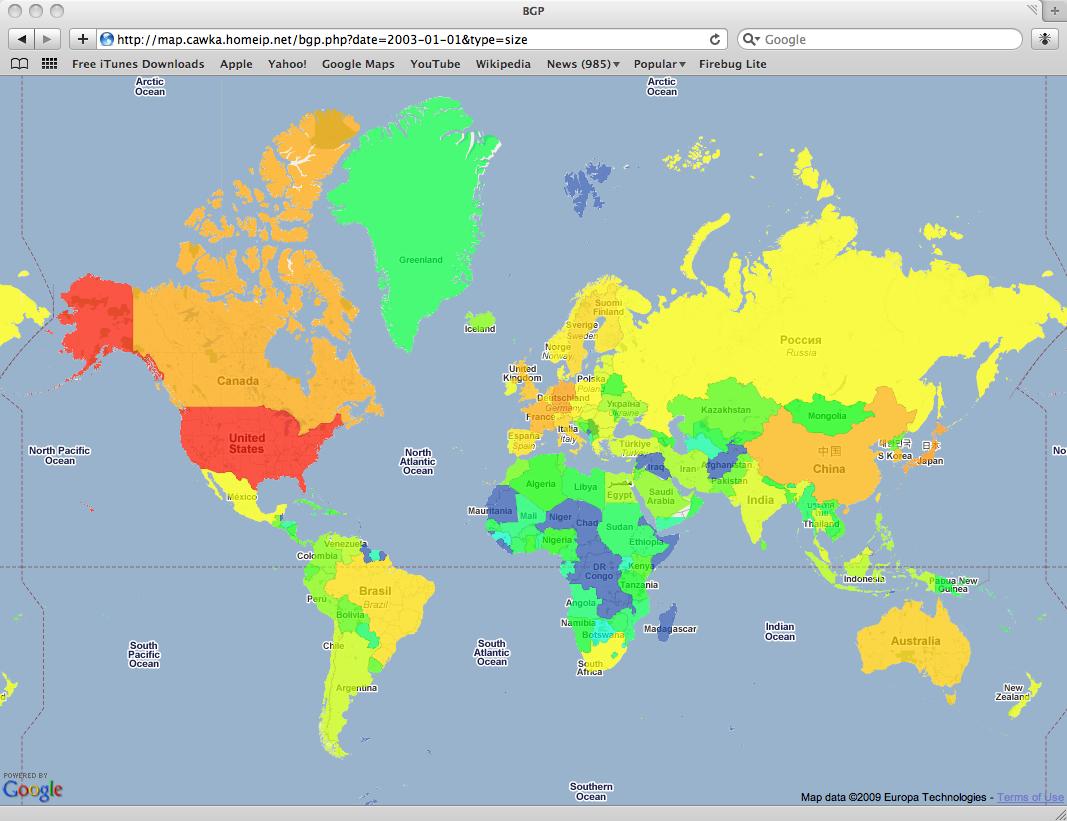
\includegraphics[trim=0 17px 0px 76px,clip=true,width=\columnwidth]{00_maps/bgp_size_2003}%
		\hspace{-0.98\columnwidth}%
		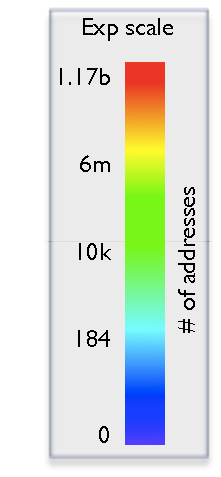
\includegraphics[width=1cm]{scale_bgp_size}\hspace{-1cm}%
		\hspace{0.98\columnwidth}
	\caption{Geographical distribution of announced IP space on \textbf{January 1, 2003}}
	\label{fig:bgp ip space 2003}
% \end{figure}
\end{minipage}%
%
\quad
%
\begin{minipage}[b]{0.48\textwidth}
% \begin{figure}[p]
	\centering
		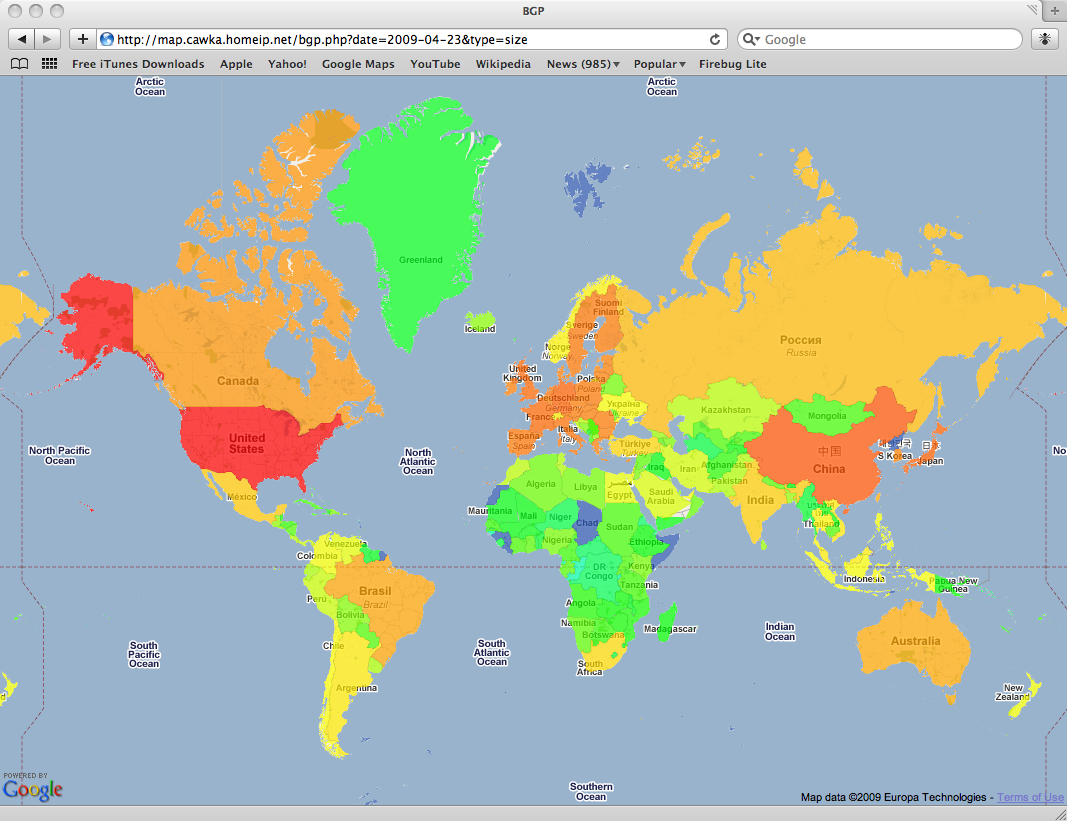
\includegraphics[trim=0 17px 0px 76px,clip=true,width=\columnwidth]{00_maps/bgp_size_2009_2}%
		\hspace{-0.98\columnwidth}%
		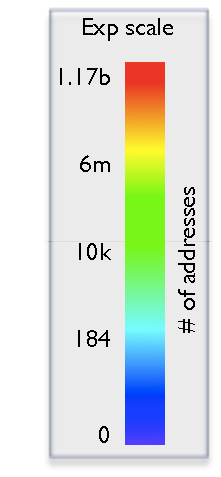
\includegraphics[width=1cm]{scale_bgp_size}\hspace{-1cm}%
		\hspace{0.98\columnwidth}
	\caption{Geographical distribution of announced IP space on \textbf{April 23, 2009}}
	\label{fig:bgp ip space 2009}
% \end{figure}
\end{minipage}

\vspace{0.5cm}

%%%%%%%%%%%%%%%%%%%%%%%%%%%%%%%%%%%%%%%%%%%%%%%%%%%%%%%%%%%%%%%%%%
%% Asia region
%%%%%%%%%%%%%%%%%%%%%%%%%%%%%%%%%%%%%%%%%%%%%%%%%%%%%%%%%%%%%%%%%%
\begin{minipage}[b]{0.48\textwidth}
% \begin{figure}[p]
	\centering
		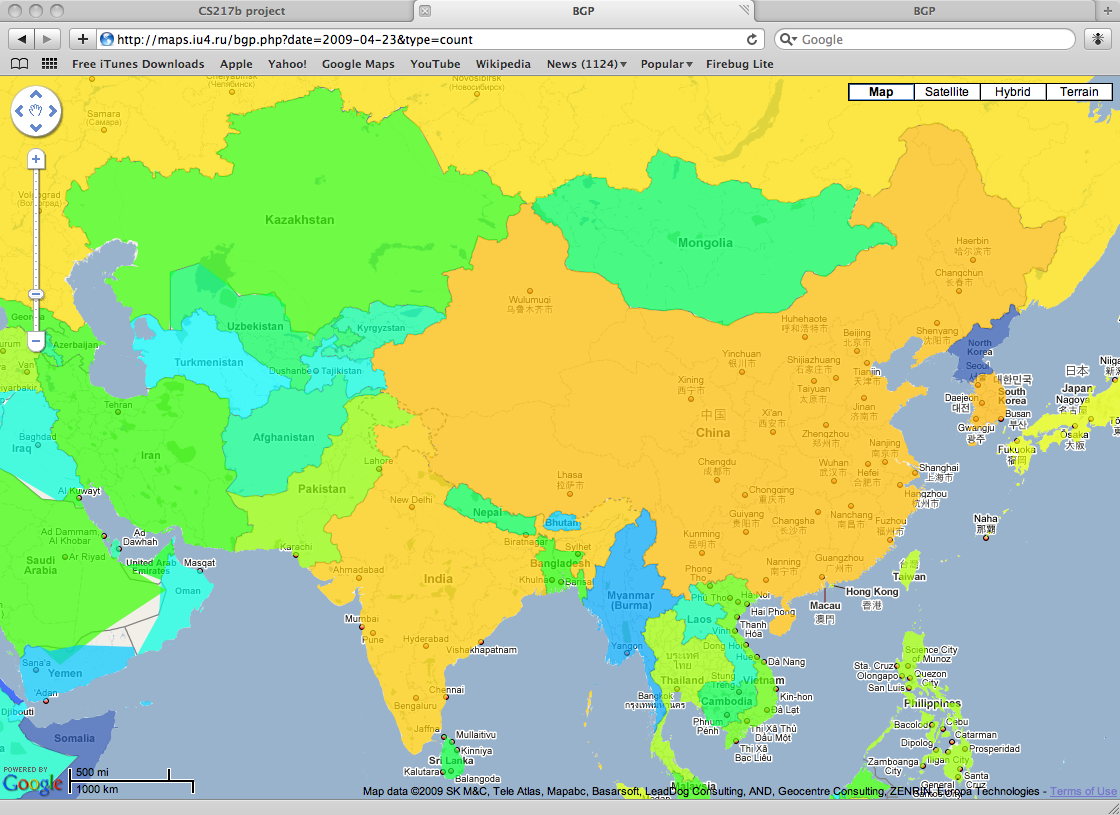
\includegraphics[trim=0 17px 0px 76px,clip=true,width=\columnwidth]{00_maps/asia_2009_prefixes}%
		\hspace{-0.98\columnwidth}%
		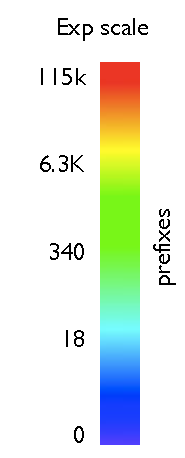
\includegraphics[width=1cm]{scale_bgp_count}\hspace{-1cm}%
		\hspace{0.98\columnwidth}
	\caption{Geographical distribution of number of announced prefixes in Asian region on \textbf{April 23, 2009}}
	\label{fig:bgp prefixes asia 2009}
% \end{figure}
\end{minipage}%
%
\quad
%
\begin{minipage}[b]{0.48\textwidth}
% \begin{figure}[p]
	\centering
		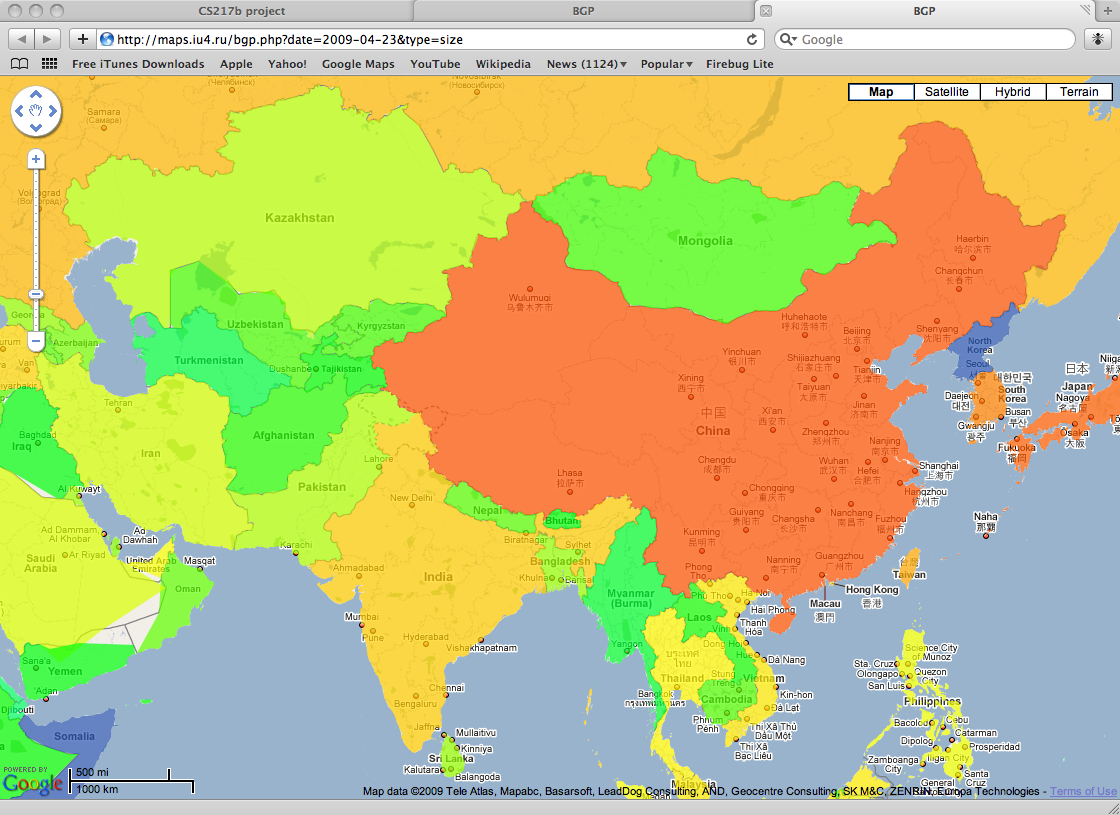
\includegraphics[trim=0 17px 0px 76px,clip=true,width=\columnwidth]{00_maps/asia_2009_space}%
		\hspace{-0.98\columnwidth}%
		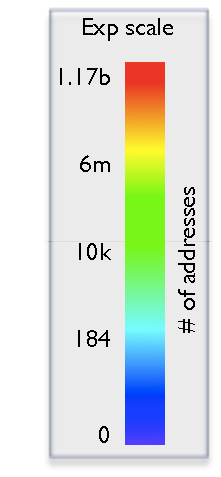
\includegraphics[width=1cm]{scale_bgp_size}\hspace{-1cm}%
		\hspace{0.98\columnwidth}
	\caption{Geographical distribution of announced IP space in Asian region on \textbf{April 23, 2009}}
	\label{fig:bgp ip space asia 2009}
% \end{figure}
\end{minipage}

\end{figure*}

% \clearpage

